\documentclass[twoside]{book}

% Packages required by doxygen
\usepackage{fixltx2e}
\usepackage{calc}
\usepackage{doxygen}
\usepackage[export]{adjustbox} % also loads graphicx
\usepackage{graphicx}
\usepackage[utf8]{inputenc}
\usepackage{makeidx}
\usepackage{multicol}
\usepackage{multirow}
\PassOptionsToPackage{warn}{textcomp}
\usepackage{textcomp}
\usepackage[nointegrals]{wasysym}
\usepackage[table]{xcolor}

% Font selection
\usepackage[T1]{fontenc}
\usepackage[scaled=.90]{helvet}
\usepackage{courier}
\usepackage{amssymb}
\usepackage{sectsty}
\renewcommand{\familydefault}{\sfdefault}
\allsectionsfont{%
  \fontseries{bc}\selectfont%
  \color{darkgray}%
}
\renewcommand{\DoxyLabelFont}{%
  \fontseries{bc}\selectfont%
  \color{darkgray}%
}
\newcommand{\+}{\discretionary{\mbox{\scriptsize$\hookleftarrow$}}{}{}}

% Page & text layout
\usepackage{geometry}
\geometry{%
  a4paper,%
  top=2.5cm,%
  bottom=2.5cm,%
  left=2.5cm,%
  right=2.5cm%
}
\tolerance=750
\hfuzz=15pt
\hbadness=750
\setlength{\emergencystretch}{15pt}
\setlength{\parindent}{0cm}
\setlength{\parskip}{3ex plus 2ex minus 2ex}
\makeatletter
\renewcommand{\paragraph}{%
  \@startsection{paragraph}{4}{0ex}{-1.0ex}{1.0ex}{%
    \normalfont\normalsize\bfseries\SS@parafont%
  }%
}
\renewcommand{\subparagraph}{%
  \@startsection{subparagraph}{5}{0ex}{-1.0ex}{1.0ex}{%
    \normalfont\normalsize\bfseries\SS@subparafont%
  }%
}
\makeatother

% Headers & footers
\usepackage{fancyhdr}
\pagestyle{fancyplain}
\fancyhead[LE]{\fancyplain{}{\bfseries\thepage}}
\fancyhead[CE]{\fancyplain{}{}}
\fancyhead[RE]{\fancyplain{}{\bfseries\leftmark}}
\fancyhead[LO]{\fancyplain{}{\bfseries\rightmark}}
\fancyhead[CO]{\fancyplain{}{}}
\fancyhead[RO]{\fancyplain{}{\bfseries\thepage}}
\fancyfoot[LE]{\fancyplain{}{}}
\fancyfoot[CE]{\fancyplain{}{}}
\fancyfoot[RE]{\fancyplain{}{\bfseries\scriptsize Generated by Doxygen }}
\fancyfoot[LO]{\fancyplain{}{\bfseries\scriptsize Generated by Doxygen }}
\fancyfoot[CO]{\fancyplain{}{}}
\fancyfoot[RO]{\fancyplain{}{}}
\renewcommand{\footrulewidth}{0.4pt}
\renewcommand{\chaptermark}[1]{%
  \markboth{#1}{}%
}
\renewcommand{\sectionmark}[1]{%
  \markright{\thesection\ #1}%
}

% Indices & bibliography
\usepackage{natbib}
\usepackage[titles]{tocloft}
\setcounter{tocdepth}{3}
\setcounter{secnumdepth}{5}
\makeindex

% Hyperlinks (required, but should be loaded last)
\usepackage{ifpdf}
\ifpdf
  \usepackage[pdftex,pagebackref=true]{hyperref}
\else
  \usepackage[ps2pdf,pagebackref=true]{hyperref}
\fi
\hypersetup{%
  colorlinks=true,%
  linkcolor=blue,%
  citecolor=blue,%
  unicode%
}

% Custom commands
\newcommand{\clearemptydoublepage}{%
  \newpage{\pagestyle{empty}\cleardoublepage}%
}

\usepackage{caption}
\captionsetup{labelsep=space,justification=centering,font={bf},singlelinecheck=off,skip=4pt,position=top}

%===== C O N T E N T S =====

\begin{document}

% Titlepage & ToC
\hypersetup{pageanchor=false,
             bookmarksnumbered=true,
             pdfencoding=unicode
            }
\pagenumbering{alph}
\begin{titlepage}
\vspace*{7cm}
\begin{center}%
{\Large P\+R\+O\+J\+E\+C\+T\+\_\+\+N\+A\+ME }\\
\vspace*{1cm}
{\large Generated by Doxygen 1.8.13}\\
\end{center}
\end{titlepage}
\clearemptydoublepage
\pagenumbering{roman}
\tableofcontents
\clearemptydoublepage
\pagenumbering{arabic}
\hypersetup{pageanchor=true}

%--- Begin generated contents ---
\chapter{CS 202 Semester Project Template}
\label{index}\hypertarget{index}{}a list of all group members the responsibilities taken on by each membera description of the design, including U\+ML diagrams and a short section on any challenges encountered in the project

Group Members and Responsiblities\+: Edward Martinez-\/\+Anaya\+: 4, 8, 16 bit processing\+: Read\+Wav, Wav Aisling Viets\+: \hyperlink{classEcho}{Echo}, \hyperlink{classProcessor}{Processor}, Metadata Claire Foy\+: Main, Limiter, \hyperlink{classNoisegate}{Noisegate}

For the design of the program, we had the main function handle user interaction and display, first asking for the .wav file that is going to be modified. It checks if the file exists and if it opens, before extracting the relevant data from the file, and displaying it to the user. It uses Read\+Wav and Wav to read and analyze the data respecively, before storing it into the appropriate categories. It asks which processor the user wants to use on the audio file. Main calls on the necessary processor, all of which inherit from the processor class, and saves the edited .wav file as a separate file.

U\+ML diagram can be viewed in repository\+: U\+ML diagram.\+jfif

Figuring out the inheritance and implementation of templates was challenging. Metadata and dealing with the different bits of audio was also difficult. Edward also couldn\textquotesingle{}t access the repository due to a 404 error every time he did. He sent us (Aisling Viets and Claire Foy) his code over discord and we pasted it into the repository for him. We indluded in our commit messages if we were committing code that Edward wrote. 
\chapter{Hierarchical Index}
\section{Class Hierarchy}
This inheritance list is sorted roughly, but not completely, alphabetically\+:\begin{DoxyCompactList}
\item \contentsline{section}{Processor}{\pageref{classProcessor}}{}
\begin{DoxyCompactList}
\item \contentsline{section}{Echo$<$ E $>$}{\pageref{classEcho}}{}
\item \contentsline{section}{Noisegate}{\pageref{classNoisegate}}{}
\item \contentsline{section}{Normalizer}{\pageref{classNormalizer}}{}
\end{DoxyCompactList}
\item \contentsline{section}{Reader}{\pageref{classReader}}{}
\item \contentsline{section}{W\+A\+V\+\_\+\+H\+E\+A\+D\+ER}{\pageref{structWAV__HEADER}}{}
\end{DoxyCompactList}

\chapter{Class Index}
\section{Class List}
Here are the classes, structs, unions and interfaces with brief descriptions\+:\begin{DoxyCompactList}
\item\contentsline{section}{\hyperlink{classEcho}{Echo$<$ E $>$} }{\pageref{classEcho}}{}
\item\contentsline{section}{\hyperlink{classNoisegate}{Noisegate} }{\pageref{classNoisegate}}{}
\item\contentsline{section}{\hyperlink{classNormalizer}{Normalizer} }{\pageref{classNormalizer}}{}
\item\contentsline{section}{\hyperlink{classProcessor}{Processor} }{\pageref{classProcessor}}{}
\item\contentsline{section}{\hyperlink{classReader}{Reader} }{\pageref{classReader}}{}
\item\contentsline{section}{\hyperlink{structWAV__HEADER}{W\+A\+V\+\_\+\+H\+E\+A\+D\+ER} }{\pageref{structWAV__HEADER}}{}
\end{DoxyCompactList}

\chapter{File Index}
\section{File List}
Here is a list of all documented files with brief descriptions\+:\begin{DoxyCompactList}
\item\contentsline{section}{{\bfseries Echo.\+h} }{\pageref{Echo_8h}}{}
\item\contentsline{section}{\hyperlink{main_8cpp}{main.\+cpp} }{\pageref{main_8cpp}}{}
\item\contentsline{section}{{\bfseries noisegate.\+h} }{\pageref{noisegate_8h}}{}
\item\contentsline{section}{{\bfseries normalizer.\+h} }{\pageref{normalizer_8h}}{}
\item\contentsline{section}{{\bfseries Processor.\+h} }{\pageref{Processor_8h}}{}
\item\contentsline{section}{{\bfseries Read\+Wav.\+h} }{\pageref{ReadWav_8h}}{}
\item\contentsline{section}{{\bfseries Wav.\+h} }{\pageref{Wav_8h}}{}
\end{DoxyCompactList}

\chapter{Class Documentation}
\hypertarget{classEcho}{}\section{Echo$<$ E $>$ Class Template Reference}
\label{classEcho}\index{Echo$<$ E $>$@{Echo$<$ E $>$}}


{\ttfamily \#include $<$Echo.\+h$>$}



Inheritance diagram for Echo$<$ E $>$\+:
\nopagebreak
\begin{figure}[H]
\begin{center}
\leavevmode
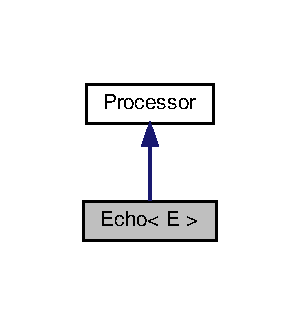
\includegraphics[width=144pt]{d1/dd3/classEcho__inherit__graph}
\end{center}
\end{figure}


Collaboration diagram for Echo$<$ E $>$\+:
\nopagebreak
\begin{figure}[H]
\begin{center}
\leavevmode
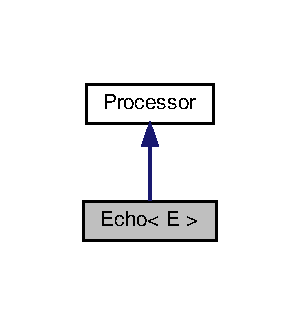
\includegraphics[width=144pt]{da/d44/classEcho__coll__graph}
\end{center}
\end{figure}
\subsection*{Public Member Functions}
\begin{DoxyCompactItemize}
\item 
\hyperlink{classEcho_a445e0cac428a957e2f4d97d28bb2ff75}{Echo} ()
\item 
void \hyperlink{classEcho_a3e23a70d522b79ef1e5b9df90c2af183}{process\+Buffer} (unsigned char $\ast$buffer, int B\+U\+F\+F\+E\+R\+\_\+\+S\+I\+ZE)
\end{DoxyCompactItemize}


\subsection{Detailed Description}
\subsubsection*{template$<$class E$>$\newline
class Echo$<$ E $>$}

This is the \hyperlink{classEcho}{Echo} class. 

\subsection{Constructor \& Destructor Documentation}
\mbox{\Hypertarget{classEcho_a445e0cac428a957e2f4d97d28bb2ff75}\label{classEcho_a445e0cac428a957e2f4d97d28bb2ff75}} 
\index{Echo@{Echo}!Echo@{Echo}}
\index{Echo@{Echo}!Echo@{Echo}}
\subsubsection{\texorpdfstring{Echo()}{Echo()}}
{\footnotesize\ttfamily template$<$class E $>$ \\
\hyperlink{classEcho}{Echo}$<$ E $>$\+::\hyperlink{classEcho}{Echo} (\begin{DoxyParamCaption}{ }\end{DoxyParamCaption})}

Individually adds 10 to the buffer values, does not allow values to exceed 32767 

\subsection{Member Function Documentation}
\mbox{\Hypertarget{classEcho_a3e23a70d522b79ef1e5b9df90c2af183}\label{classEcho_a3e23a70d522b79ef1e5b9df90c2af183}} 
\index{Echo@{Echo}!process\+Buffer@{process\+Buffer}}
\index{process\+Buffer@{process\+Buffer}!Echo@{Echo}}
\subsubsection{\texorpdfstring{process\+Buffer()}{processBuffer()}}
{\footnotesize\ttfamily template$<$class E $>$ \\
void \hyperlink{classEcho}{Echo}$<$ E $>$\+::process\+Buffer (\begin{DoxyParamCaption}\item[{unsigned char $\ast$}]{buffer,  }\item[{int}]{B\+U\+F\+F\+E\+R\+\_\+\+S\+I\+ZE }\end{DoxyParamCaption})\hspace{0.3cm}{\ttfamily [virtual]}}

Uses process\+Buffer to get buffer data and size for processing 
\begin{DoxyParams}{Parameters}
{\em buffer} & -\/ contains .wav file Data, array of unsigned char$\ast$ \\
\hline
{\em B\+U\+F\+F\+E\+R\+\_\+\+S\+I\+ZE} & -\/ contains size of buffer, integer \\
\hline
\end{DoxyParams}


Implements \hyperlink{classProcessor_a13e6240144c7a530079b0e2ae4a4526d}{Processor}.



The documentation for this class was generated from the following files\+:\begin{DoxyCompactItemize}
\item 
Echo.\+h\item 
Echo.\+cpp\end{DoxyCompactItemize}

\hypertarget{classNoisegate}{}\section{Noisegate Class Reference}
\label{classNoisegate}\index{Noisegate@{Noisegate}}


Inheritance diagram for Noisegate\+:
% FIG 0


Collaboration diagram for Noisegate\+:
% FIG 1
\subsection*{Public Member Functions}
\begin{DoxyCompactItemize}
\item 
\hyperlink{classNoisegate_a15c5621437e7378814c69a58fc60b326}{Noisegate} ()
\item 
\hyperlink{classNoisegate_a4dc5881a80f29ebc6e9be12dae2bd632}{Noisegate} (float new\+Threshold)
\item 
{\footnotesize template$<$typename T $>$ }\\void \hyperlink{classNoisegate_aee5ff92d38286e509055fa6d117415fd}{process\+Buffer} (T buffer, int buffer\+Size)
\end{DoxyCompactItemize}


\subsection{Constructor \& Destructor Documentation}
\mbox{\Hypertarget{classNoisegate_a15c5621437e7378814c69a58fc60b326}\label{classNoisegate_a15c5621437e7378814c69a58fc60b326}} 
\index{Noisegate@{Noisegate}!Noisegate@{Noisegate}}
\index{Noisegate@{Noisegate}!Noisegate@{Noisegate}}
\subsubsection{\texorpdfstring{Noisegate()}{Noisegate()}\hspace{0.1cm}{\footnotesize\ttfamily [1/2]}}
{\footnotesize\ttfamily Noisegate\+::\+Noisegate (\begin{DoxyParamCaption}{ }\end{DoxyParamCaption})}

constructor for \hyperlink{classNoisegate}{Noisegate} class \mbox{\Hypertarget{classNoisegate_a4dc5881a80f29ebc6e9be12dae2bd632}\label{classNoisegate_a4dc5881a80f29ebc6e9be12dae2bd632}} 
\index{Noisegate@{Noisegate}!Noisegate@{Noisegate}}
\index{Noisegate@{Noisegate}!Noisegate@{Noisegate}}
\subsubsection{\texorpdfstring{Noisegate()}{Noisegate()}\hspace{0.1cm}{\footnotesize\ttfamily [2/2]}}
{\footnotesize\ttfamily Noisegate\+::\+Noisegate (\begin{DoxyParamCaption}\item[{float}]{new\+Threshold }\end{DoxyParamCaption})}

parmaterized constructor for \hyperlink{classNoisegate}{Noisegate} 
\begin{DoxyParams}{Parameters}
{\em name-\/new\+Threshold-\/} & multiplier for what the max min amp can be \\
\hline
\end{DoxyParams}


\subsection{Member Function Documentation}
\mbox{\Hypertarget{classNoisegate_aee5ff92d38286e509055fa6d117415fd}\label{classNoisegate_aee5ff92d38286e509055fa6d117415fd}} 
\index{Noisegate@{Noisegate}!process\+Buffer@{process\+Buffer}}
\index{process\+Buffer@{process\+Buffer}!Noisegate@{Noisegate}}
\subsubsection{\texorpdfstring{process\+Buffer()}{processBuffer()}}
{\footnotesize\ttfamily template$<$typename T $>$ \\
void Noisegate\+::process\+Buffer (\begin{DoxyParamCaption}\item[{T}]{buffer,  }\item[{int}]{buffer\+Size }\end{DoxyParamCaption})\hspace{0.3cm}{\ttfamily [inline]}}

templated noisegate to handle different types of audio 
\begin{DoxyParams}{Parameters}
{\em name} & -\/ buffer -\/ of templated type T \\
\hline
{\em name-\/} & buffersize-\/ sent in buffer size \\
\hline
\end{DoxyParams}


The documentation for this class was generated from the following files\+:\begin{DoxyCompactItemize}
\item 
noisegate.\+h\item 
noisegate.\+cpp\end{DoxyCompactItemize}

\hypertarget{classNormalizer}{}\section{Normalizer Class Reference}
\label{classNormalizer}\index{Normalizer@{Normalizer}}


Inheritance diagram for Normalizer\+:
% FIG 0


Collaboration diagram for Normalizer\+:
% FIG 1
\subsection*{Public Member Functions}
\begin{DoxyCompactItemize}
\item 
\hyperlink{classNormalizer_af576151323854ff0d4d7e37255c397d1}{Normalizer} ()
\item 
{\footnotesize template$<$typename T $>$ }\\void \hyperlink{classNormalizer_aaef27fc4d06b2d51a1c17e349ca9ab85}{process\+Buffer} (T buffer, int buffer\+Size)
\end{DoxyCompactItemize}


\subsection{Constructor \& Destructor Documentation}
\mbox{\Hypertarget{classNormalizer_af576151323854ff0d4d7e37255c397d1}\label{classNormalizer_af576151323854ff0d4d7e37255c397d1}} 
\index{Normalizer@{Normalizer}!Normalizer@{Normalizer}}
\index{Normalizer@{Normalizer}!Normalizer@{Normalizer}}
\subsubsection{\texorpdfstring{Normalizer()}{Normalizer()}}
{\footnotesize\ttfamily Normalizer\+::\+Normalizer (\begin{DoxyParamCaption}{ }\end{DoxyParamCaption})}

constructor for \hyperlink{classNormalizer}{Normalizer} class 

\subsection{Member Function Documentation}
\mbox{\Hypertarget{classNormalizer_aaef27fc4d06b2d51a1c17e349ca9ab85}\label{classNormalizer_aaef27fc4d06b2d51a1c17e349ca9ab85}} 
\index{Normalizer@{Normalizer}!process\+Buffer@{process\+Buffer}}
\index{process\+Buffer@{process\+Buffer}!Normalizer@{Normalizer}}
\subsubsection{\texorpdfstring{process\+Buffer()}{processBuffer()}}
{\footnotesize\ttfamily template$<$typename T $>$ \\
void Normalizer\+::process\+Buffer (\begin{DoxyParamCaption}\item[{T}]{buffer,  }\item[{int}]{buffer\+Size }\end{DoxyParamCaption})\hspace{0.3cm}{\ttfamily [inline]}}

templated normalizer to handle different types of audio 
\begin{DoxyParams}{Parameters}
{\em name} & -\/ buffer -\/ of templated type T \\
\hline
{\em name-\/} & buffersize-\/ sent in buffer size \\
\hline
\end{DoxyParams}


The documentation for this class was generated from the following files\+:\begin{DoxyCompactItemize}
\item 
normalizer.\+h\item 
normalizer.\+cpp\end{DoxyCompactItemize}

\hypertarget{classProcessor}{}\section{Processor Class Reference}
\label{classProcessor}\index{Processor@{Processor}}


{\ttfamily \#include $<$Processor.\+h$>$}



Inheritance diagram for Processor\+:
\nopagebreak
\begin{figure}[H]
\begin{center}
\leavevmode
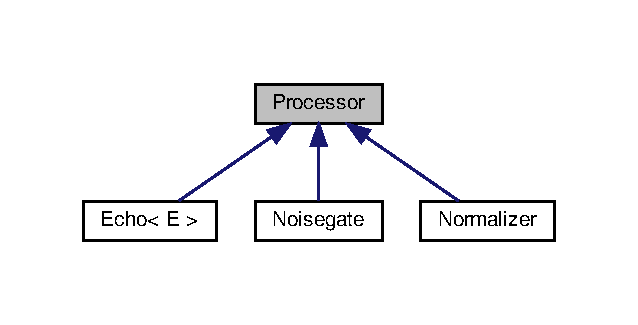
\includegraphics[width=306pt]{dd/d93/classProcessor__inherit__graph}
\end{center}
\end{figure}
\subsection*{Public Member Functions}
\begin{DoxyCompactItemize}
\item 
virtual void \hyperlink{classProcessor_a13e6240144c7a530079b0e2ae4a4526d}{process\+Buffer} (unsigned char $\ast$buffer, int B\+U\+F\+F\+E\+R\+\_\+\+S\+I\+ZE)=0
\end{DoxyCompactItemize}


\subsection{Detailed Description}
This is the \hyperlink{classProcessor}{Processor} class (virtual, abstract). 

\subsection{Member Function Documentation}
\mbox{\Hypertarget{classProcessor_a13e6240144c7a530079b0e2ae4a4526d}\label{classProcessor_a13e6240144c7a530079b0e2ae4a4526d}} 
\index{Processor@{Processor}!process\+Buffer@{process\+Buffer}}
\index{process\+Buffer@{process\+Buffer}!Processor@{Processor}}
\subsubsection{\texorpdfstring{process\+Buffer()}{processBuffer()}}
{\footnotesize\ttfamily virtual void Processor\+::process\+Buffer (\begin{DoxyParamCaption}\item[{unsigned char $\ast$}]{buffer,  }\item[{int}]{B\+U\+F\+F\+E\+R\+\_\+\+S\+I\+ZE }\end{DoxyParamCaption})\hspace{0.3cm}{\ttfamily [pure virtual]}}

Gets buffer data and size to pass to classes which inherit from \hyperlink{classProcessor}{Processor} 
\begin{DoxyParams}{Parameters}
{\em buffer} & -\/ contains .wav file Data, array of unsigned char$\ast$ \\
\hline
{\em B\+U\+F\+F\+E\+R\+\_\+\+S\+I\+ZE} & -\/ contains size of buffer, integer \\
\hline
\end{DoxyParams}


Implemented in \hyperlink{classEcho_a3e23a70d522b79ef1e5b9df90c2af183}{Echo$<$ E $>$}.



The documentation for this class was generated from the following file\+:\begin{DoxyCompactItemize}
\item 
Processor.\+h\end{DoxyCompactItemize}

\hypertarget{classReader}{}\section{Reader Class Reference}
\label{classReader}\index{Reader@{Reader}}
\subsection*{Public Member Functions}
\begin{DoxyCompactItemize}
\item 
\mbox{\Hypertarget{classReader_a7cd76dec58af34626d0d7f928d077773}\label{classReader_a7cd76dec58af34626d0d7f928d077773}} 
{\bfseries Reader} (F\+I\+LE $\ast$)
\item 
void \hyperlink{classReader_aa33ad038bf60829bd30149a5b8436bb2}{Read\+Wav} (F\+I\+LE $\ast$)
\item 
int \hyperlink{classReader_a26e7eb6fabd4424304d00658907a4878}{get\+File\+Size} (F\+I\+LE $\ast$in\+File)
\item 
unsigned char $\ast$ \hyperlink{classReader_a5cc512699b1ae2e13186977ccdffe8f7}{get\+Buffer} ()
\item 
int \hyperlink{classReader_af56ef824ae4f49fb6cfc89d7443e9ede}{get\+Buffer\+Size} () const
\end{DoxyCompactItemize}


\subsection{Member Function Documentation}
\mbox{\Hypertarget{classReader_a5cc512699b1ae2e13186977ccdffe8f7}\label{classReader_a5cc512699b1ae2e13186977ccdffe8f7}} 
\index{Reader@{Reader}!get\+Buffer@{get\+Buffer}}
\index{get\+Buffer@{get\+Buffer}!Reader@{Reader}}
\subsubsection{\texorpdfstring{get\+Buffer()}{getBuffer()}}
{\footnotesize\ttfamily unsigned char$\ast$ Reader\+::get\+Buffer (\begin{DoxyParamCaption}{ }\end{DoxyParamCaption})}

The function returns the buffer after being called \mbox{\Hypertarget{classReader_af56ef824ae4f49fb6cfc89d7443e9ede}\label{classReader_af56ef824ae4f49fb6cfc89d7443e9ede}} 
\index{Reader@{Reader}!get\+Buffer\+Size@{get\+Buffer\+Size}}
\index{get\+Buffer\+Size@{get\+Buffer\+Size}!Reader@{Reader}}
\subsubsection{\texorpdfstring{get\+Buffer\+Size()}{getBufferSize()}}
{\footnotesize\ttfamily int Reader\+::get\+Buffer\+Size (\begin{DoxyParamCaption}{ }\end{DoxyParamCaption}) const}

The function calls in the Wav\+Header struct and pulls the bits per sample variable to determine buffer type \mbox{\Hypertarget{classReader_a26e7eb6fabd4424304d00658907a4878}\label{classReader_a26e7eb6fabd4424304d00658907a4878}} 
\index{Reader@{Reader}!get\+File\+Size@{get\+File\+Size}}
\index{get\+File\+Size@{get\+File\+Size}!Reader@{Reader}}
\subsubsection{\texorpdfstring{get\+File\+Size()}{getFileSize()}}
{\footnotesize\ttfamily int Reader\+::get\+File\+Size (\begin{DoxyParamCaption}\item[{F\+I\+LE $\ast$}]{in\+File }\end{DoxyParamCaption})}

Reads in a F\+I\+LE pointer to get the size fo the wav file 
\begin{DoxyParams}{Parameters}
{\em F\+I\+LE} & pointer to determine size of audio file \\
\hline
\end{DoxyParams}
\mbox{\Hypertarget{classReader_aa33ad038bf60829bd30149a5b8436bb2}\label{classReader_aa33ad038bf60829bd30149a5b8436bb2}} 
\index{Reader@{Reader}!Read\+Wav@{Read\+Wav}}
\index{Read\+Wav@{Read\+Wav}!Reader@{Reader}}
\subsubsection{\texorpdfstring{Read\+Wav()}{ReadWav()}}
{\footnotesize\ttfamily void Reader\+::\+Read\+Wav (\begin{DoxyParamCaption}\item[{F\+I\+LE $\ast$}]{wav\+File }\end{DoxyParamCaption})}

Takes in a F\+I\+LE pointer of the audio data and displays the information 
\begin{DoxyParams}{Parameters}
{\em the} & audio wav data as a F\+I\+LE Pointer \\
\hline
\end{DoxyParams}


The documentation for this class was generated from the following files\+:\begin{DoxyCompactItemize}
\item 
Read\+Wav.\+h\item 
Read\+Wav.\+cpp\end{DoxyCompactItemize}

\hypertarget{structWAV__HEADER}{}\section{W\+A\+V\+\_\+\+H\+E\+A\+D\+ER Struct Reference}
\label{structWAV__HEADER}\index{W\+A\+V\+\_\+\+H\+E\+A\+D\+ER@{W\+A\+V\+\_\+\+H\+E\+A\+D\+ER}}
\subsection*{Public Attributes}
\begin{DoxyCompactItemize}
\item 
\mbox{\Hypertarget{structWAV__HEADER_a8406498dfbcaaff8823f926554b0b5ae}\label{structWAV__HEADER_a8406498dfbcaaff8823f926554b0b5ae}} 
char {\bfseries R\+I\+FF} \mbox{[}4\mbox{]}
\item 
\mbox{\Hypertarget{structWAV__HEADER_aec71b96ceea4b1767543db830999b716}\label{structWAV__HEADER_aec71b96ceea4b1767543db830999b716}} 
int {\bfseries Chunk\+Size}
\item 
\mbox{\Hypertarget{structWAV__HEADER_a52a80583ba9282a799dc60888d4cee92}\label{structWAV__HEADER_a52a80583ba9282a799dc60888d4cee92}} 
char {\bfseries W\+A\+VE} \mbox{[}4\mbox{]}
\item 
\mbox{\Hypertarget{structWAV__HEADER_a4720b4ea78fe5c0ce5bfc29cc90d4c86}\label{structWAV__HEADER_a4720b4ea78fe5c0ce5bfc29cc90d4c86}} 
char {\bfseries Format} \mbox{[}4\mbox{]}
\item 
\mbox{\Hypertarget{structWAV__HEADER_a35e7322433e76c8e53ad7f12205db141}\label{structWAV__HEADER_a35e7322433e76c8e53ad7f12205db141}} 
int {\bfseries Chunk1\+Size}
\item 
\mbox{\Hypertarget{structWAV__HEADER_a694117914b2333a5b07e667ad0dae617}\label{structWAV__HEADER_a694117914b2333a5b07e667ad0dae617}} 
short {\bfseries Audio\+Format}
\item 
\mbox{\Hypertarget{structWAV__HEADER_a6bf86bc189b27c2c9ac4541792fc9aee}\label{structWAV__HEADER_a6bf86bc189b27c2c9ac4541792fc9aee}} 
short {\bfseries Number\+Of\+Channels}
\item 
\mbox{\Hypertarget{structWAV__HEADER_a055f847201c7104f1f366d5d32d7d1de}\label{structWAV__HEADER_a055f847201c7104f1f366d5d32d7d1de}} 
int {\bfseries Sample\+Rate}
\item 
\mbox{\Hypertarget{structWAV__HEADER_afde112165ca94b23cc4e614eab2ce9d1}\label{structWAV__HEADER_afde112165ca94b23cc4e614eab2ce9d1}} 
int {\bfseries Byte\+Rate}
\item 
\mbox{\Hypertarget{structWAV__HEADER_aa3ef0f6569986a915ddc0f71adc29746}\label{structWAV__HEADER_aa3ef0f6569986a915ddc0f71adc29746}} 
short {\bfseries Sample\+Alignment}
\item 
\mbox{\Hypertarget{structWAV__HEADER_a2d07ad1e8f9cc4283fe815f2e19280fb}\label{structWAV__HEADER_a2d07ad1e8f9cc4283fe815f2e19280fb}} 
short {\bfseries Bits\+Per\+Sample}
\item 
\mbox{\Hypertarget{structWAV__HEADER_a1f3735cd90aaa9fc7cfb2b91c8244359}\label{structWAV__HEADER_a1f3735cd90aaa9fc7cfb2b91c8244359}} 
char {\bfseries Sub\+Chunk2\+ID} \mbox{[}4\mbox{]}
\item 
\mbox{\Hypertarget{structWAV__HEADER_afe043c070454cc67517fab9a5d21cbbc}\label{structWAV__HEADER_afe043c070454cc67517fab9a5d21cbbc}} 
int {\bfseries Sub\+Chunk2\+Size}
\end{DoxyCompactItemize}


The documentation for this struct was generated from the following file\+:\begin{DoxyCompactItemize}
\item 
Wav.\+h\end{DoxyCompactItemize}

\chapter{File Documentation}
\hypertarget{main_8cpp}{}\section{main.\+cpp File Reference}
\label{main_8cpp}\index{main.\+cpp@{main.\+cpp}}
{\ttfamily \#include \char`\"{}Wav.\+h\char`\"{}}\newline
{\ttfamily \#include \char`\"{}Read\+Wav.\+h\char`\"{}}\newline
{\ttfamily \#include \char`\"{}Processor.\+h\char`\"{}}\newline
{\ttfamily \#include \char`\"{}Echo.\+h\char`\"{}}\newline
{\ttfamily \#include \char`\"{}noisegate.\+h\char`\"{}}\newline
{\ttfamily \#include \char`\"{}normalizer.\+h\char`\"{}}\newline
{\ttfamily \#include $<$iostream$>$}\newline
Include dependency graph for main.\+cpp\+:

%--- End generated contents ---

% Index
\backmatter
\newpage
\phantomsection
\clearemptydoublepage
\addcontentsline{toc}{chapter}{Index}
\printindex

\end{document}
